\documentclass{article}

\usepackage[letterpaper]{geometry}
\usepackage{amsmath}
\usepackage{siunitx}
\usepackage{graphicx}

\title{4261 HW 7}
\author{Duncan Wilkie}
\date{}

\begin{document}

\maketitle

\section{}
In the tight-binding and nearly-free electron models, one observes discontinuities in the dispersion plot at the Brillouin zone boundaries.
Connected components of the dispersion plot are called bands.
Sodium is in group I, and as such has a half-filled valence band, making it a metal, because if a Coulomb potential is applied, the electron
from one atom is free to move to the opposite-spin state in the other half of the valence band on its neighbor, i.e. it's conductive.
Calcium, in group II, has valence 2, so one might think it's an insulator.
However, it is possible for the potential to be such that the band energies overlap, and one electron half-fills the valence band
while the other goes into the conduction band.
Evidently, this occurs for calcium.
Carbon, silicon, and germanium are all group IV, and so one would expect the valence electrons to form two completely filled bands.
Indeed this is the case; it just so happens that the band gaps in silicon and germanium are sufficiently smaller than diamond to make
the latter an insulator and the others semiconductors.
Diamond is transparent because its insulating nature means that incident light cannot excite the electrons unless the photons are
sufficiently energetic to move them to the conduction band.
It so happens that diamond's band gap is sufficiently large that the excitation frequencies are higher than those of visible light, so
visible light doesn't interact with the atoms in the crystal, and it is transparent.

\section{}
A sketch of the given dispersion in the extended zone scheme with $k_{x}=k_{y}$ appears below.
\[
  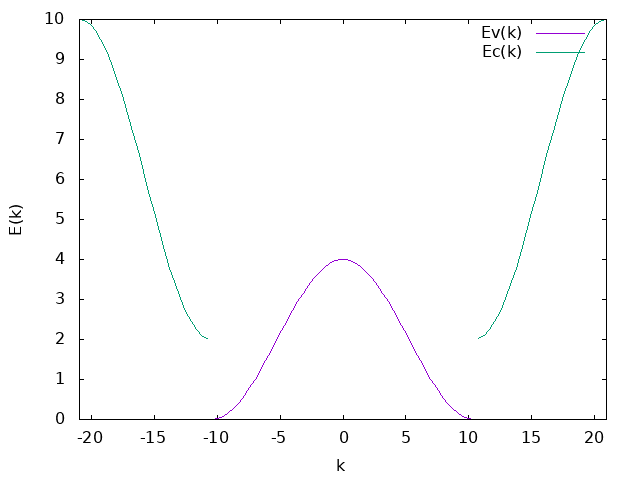
\includegraphics[scale=.8]{plot1.png}
\]
The band gap clearly occurs at the Brillouin zone boundary, in this case $\pm \pi/0.3$, and has magnitude
\[
  \epsilon_{c}(0)-\epsilon_{v}(\pi/0.3)=\SI{2}{eV}-\SI{0}{eV}=\SI{2}{eV}
\]
Near the band edges, we may approximate $\cos(k_{x}a)\approx 1-k_{x}^{2}a^{2}/2$ and $\cos(k_{y}a)\approx 1-k_{y}^{2}a^{2}/2$ to get
\[
  \epsilon_{c}(\vec{k})=c\Rightarrow 6-2(1-k_{x}^{2}a^{2}/2+1-k_{y}^{2}a^{2}/2)=c
  \Rightarrow k_{x}^{2}+k_{y}^{2}=c_{1}^{2}
\]
and
\[
  \epsilon_{v}(\vec{k})=c \Rightarrow 2+(1-k_{x}^{2}a^{2}/2+1-k_{y}^{2}a^{2}/2)
  \Rightarrow k_{x}^{2}+k_{y}^{2}= c_{2}^{2}
\]
which are the equations for $k$-space circles.
In the language of the effective mass section, we have $\alpha=a^{2}/2$ (using the expansion of cosine about its minimum) from which we can find the effective mass via
\[
  \frac{\hbar^{2}}{m^{*}}=2\alpha
  \Leftrightarrow m^{*}=\frac{\hbar^{2}}{2(a^{2}/2)}=\frac{\hbar^{2}}{a^{2}}
  =\frac{(\SI{1.05e-34}{J\cdot s})^{2}}{(\SI{0.3}{nm})^{2}}
  =\SI{1.23e-49}{kg}
\]
The effective mass of the holes is equal to this (since the expansion of cosine about its maximum and minimum have the same second term
have the same magnitude, but different sign; the term is negated in the computation of $m^{*}$).
Using the expressions derived in the book,
\[
  g_{c}(\epsilon\geq \epsilon_{c})=\frac{(2m_{e}^{*})^{3/2}}{2\pi^{2}\hbar^{3}}\sqrt{\epsilon-\epsilon_{cz}}
\]
and
\[
  g_{v}(\epsilon\leq \epsilon_{v})=\frac{(2m_{h}^{*})^{3/2}}{2\pi^{2}\hbar^{3}}\sqrt{\epsilon_{v}-\epsilon}
\]
Plotting these, % TODO: plot, see if extension necessary
% TODO: tight-binding Hamiltonian
\section*{}
\end{document}
%%% Local Variables:
%%% mode: latex
%%% TeX-master: t
%%% End:
